\documentclass{standalone}

\usepackage{tikz}
\usetikzlibrary{arrows}
\usetikzlibrary{decorations.markings}

\begin{document}

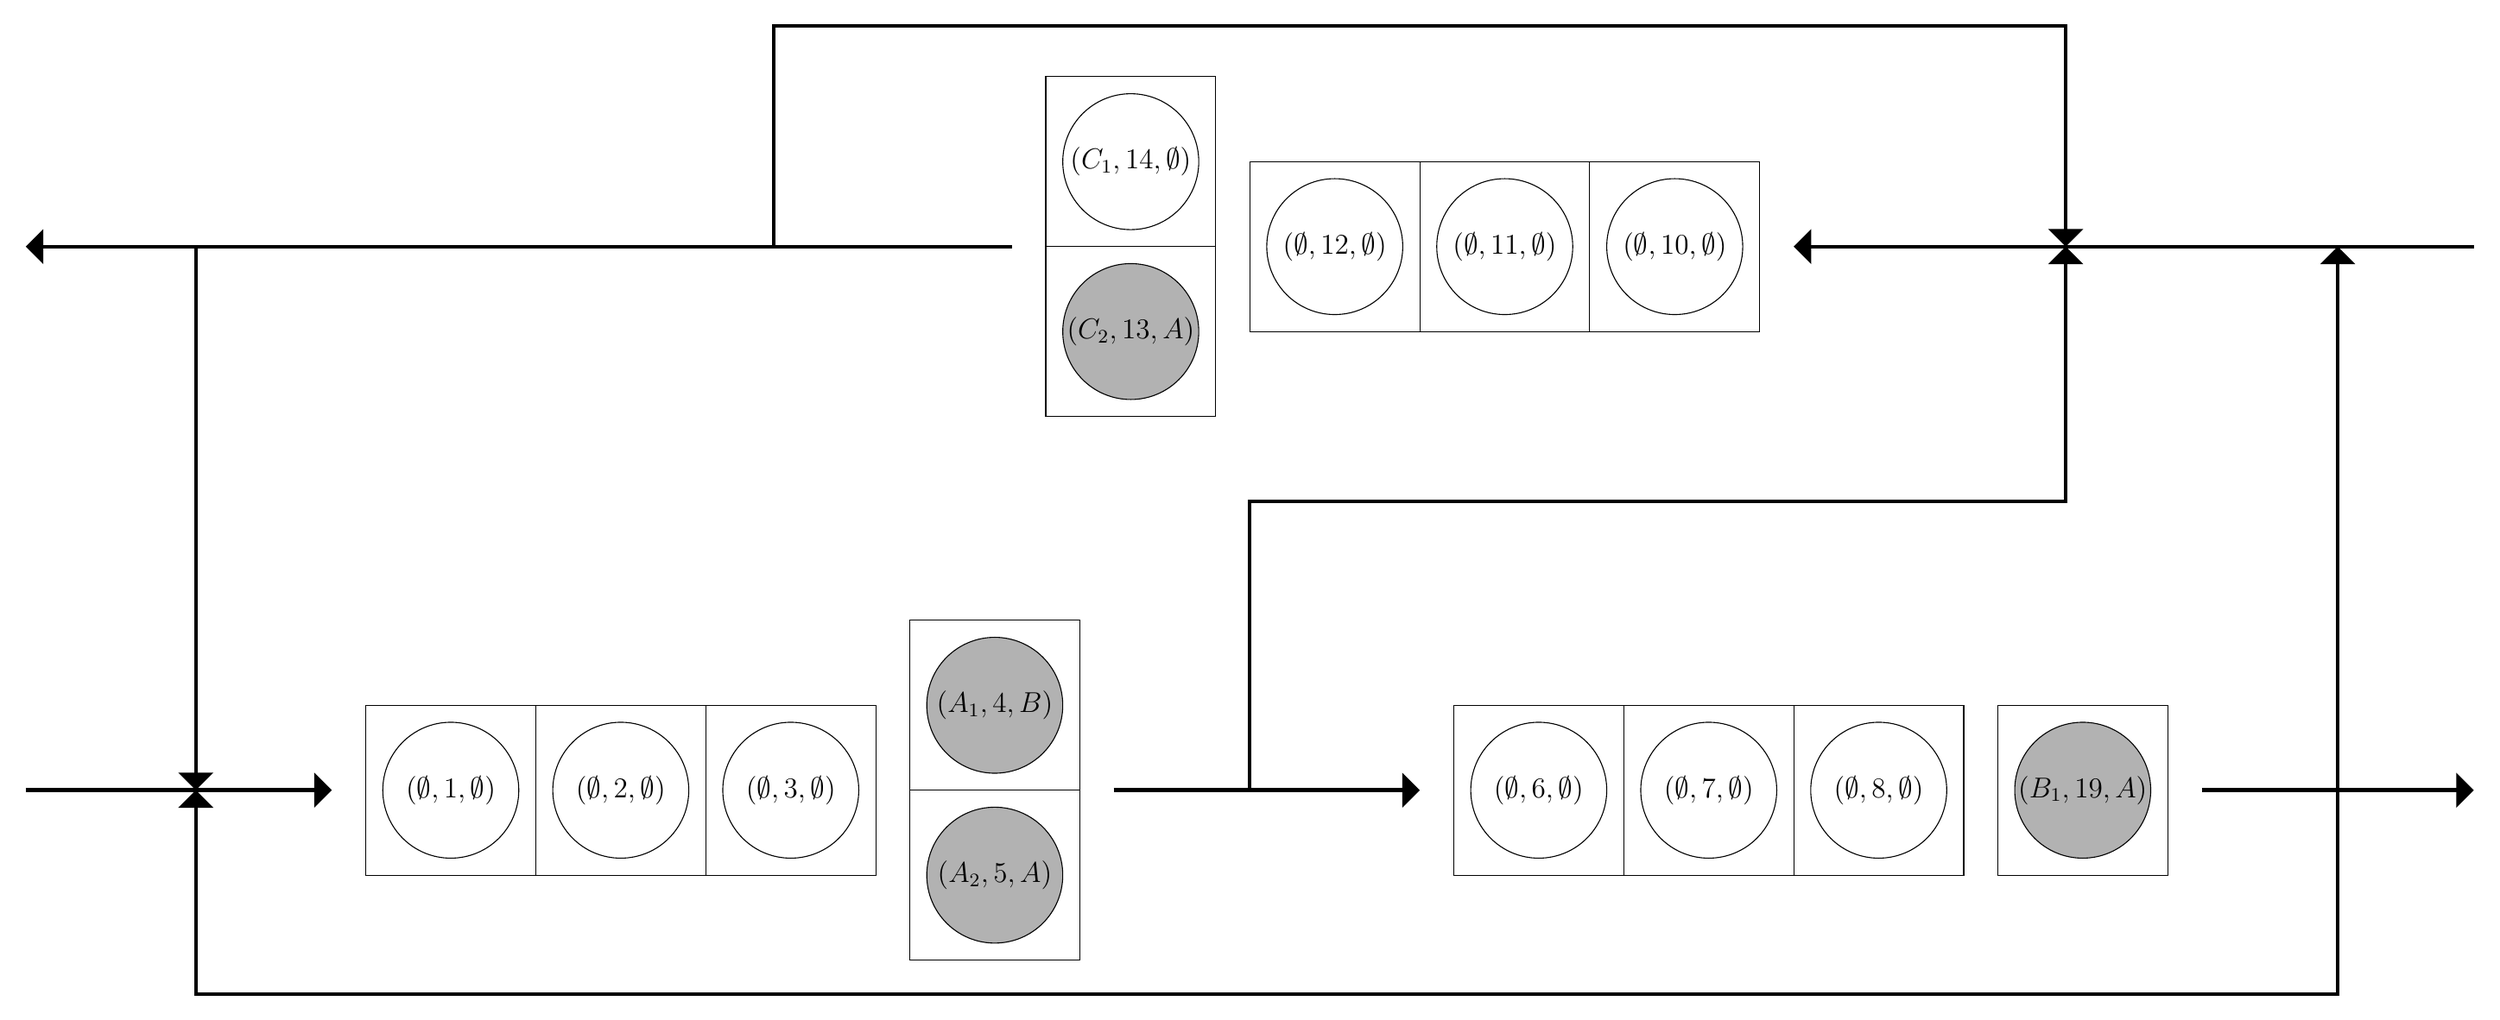
\begin{tikzpicture}
  % Queue A
  \draw (0, 0) -- (2.5, 0) -- (2.5, 2.5) -- (0, 2.5) -- cycle;
  \draw (2.5, 0) -- (2.5, 2.5) -- (5, 2.5) -- (5, 0) -- cycle;
  \draw (7.5, 0) -- (7.5, 2.5) -- (5, 2.5) -- (5, 0) -- cycle;

  % Service center A
  \draw (8, -1.25) -- (8, 1.25) -- (10.5, 1.25) -- (10.5, -1.25) -- cycle;
  \draw (8, 1.25) -- (8, 3.75) -- (10.5, 3.75) -- (10.5, 1.25) -- cycle;

  % Queue B
  \draw (16, 0) -- (18.5, 0) -- (18.5, 2.5) -- (16, 2.5) -- cycle;
  \draw (18.5, 0) -- (18.5, 2.5) -- (21, 2.5) -- (21, 0) -- cycle;
  \draw (23.5, 0) -- (23.5, 2.5) -- (21, 2.5) -- (21, 0) -- cycle;

  % Service center B
  \draw (24, 0) -- (24, 2.5) -- (26.5, 2.5) -- (26.5, 0) -- cycle;

  % Queue C
  \draw (13, 8) -- (15.5, 8) -- (15.5, 10.5) -- (13, 10.5) -- cycle;
  \draw (15.5, 8) -- (18, 8) -- (18, 10.5) -- (15.5, 10.5) -- cycle;
  \draw (18, 8) -- (20.5, 8) -- (20.5, 10.5) -- (18, 10.5) -- cycle;

  % Service centre C
  \draw (10, 6.75) -- (10, 9.25) -- (12.5, 9.25) -- (12.5, 6.75) -- cycle;
  \draw (10, 9.25) -- (10, 11.75) -- (12.5, 11.75) -- (12.5, 9.25) -- cycle;

  % Routings

  \draw[ultra thick, -triangle 90] (-5, 1.25) -- (-0.5, 1.25); % Into A
  \draw[ultra thick, -triangle 90] (11, 1.25) -- (15.5, 1.25); % From A to B
  \draw[ultra thick, -triangle 90] (27, 1.25) -- (31, 1.25); % Out of B
  \draw[ultra thick, -triangle 90] (31, 9.25) -- (21, 9.25); % Into C
  \draw[ultra thick, -triangle 90] (9.5, 9.25) -- (-5, 9.25); % Out of C
  \draw[ultra thick, -triangle 90] (29, 1.25) -- (29, 9.25); % From B to C
  \draw[ultra thick, -triangle 90] (-2.5, 9.25) -- (-2.5, 1.25); % From C to A
  \draw[ultra thick, -triangle 90] (13, 1.25) -- (13, 5.5) -- (25, 5.5) -- (25, 9.25); % From A to C
  \draw[ultra thick, -triangle 90] (29, 1.25) -- (29, -1.75) -- (-2.5, -1.75) -- (-2.5, 1.25); % From B to A
  \draw[ultra thick, -triangle 90] (6, 9.25) -- (6, 12.5) -- (25, 12.5) -- (25, 9.25); % From C into itself


  % Customers waiting at A
  \draw (1.25, 1.25) circle (1) node {\large{$(\emptyset, 1, \emptyset)$}}; % Back of A
  \draw (3.75, 1.25) circle (1) node {\large{$(\emptyset, 2, \emptyset)$}}; % Middle of A
  \draw (6.25, 1.25) circle (1) node {\large{$(\emptyset, 3, \emptyset)$}}; % Front of A
  \draw[fill=black!30] (9.25, 2.5) circle (1) node {\large{$(A_1, 4, B)$}}; % Servcie top A
  \draw[fill=black!30] (9.25, 0) circle (1) node {\large{$(A_2, 5, A)$}}; % Service bottom A
  \draw (17.25, 1.25) circle (1) node {\large{$(\emptyset, 6, \emptyset)$}}; % Back of B
  \draw (19.75, 1.25) circle (1) node {\large{$(\emptyset, 7, \emptyset)$}}; % Middle of B
  \draw (22.25, 1.25) circle (1) node {\large{$(\emptyset, 8, \emptyset)$}}; % Front of B
  \draw[fill=black!30] (25.25, 1.25) circle (1) node {\large{$(B_1, 19, A)$}}; % Service B
  \draw (14.25, 9.25) circle (1) node {\large{$(\emptyset, 12, \emptyset)$}}; % Front of C
  \draw (16.75, 9.25) circle (1) node {\large{$(\emptyset, 11, \emptyset)$}}; % Middle of C
  \draw (19.25, 9.25) circle (1) node {\large{$(\emptyset, 10, \emptyset)$}}; % Back of C
  \draw[fill=black!30] (11.25, 8) circle (1) node {\large{$(C_2, 13, A)$}}; % Service bottom C
  \draw (11.25, 10.5) circle (1) node {\large{$(C_1, 14, \emptyset)$}}; % Service top C


\end{tikzpicture}

\end{document}
